%% ----------------------------------------------------------------
%% Thesis.tex -- MAIN FILE (the one that you compile with LaTeX)
%% ---------------------------------------------------------------- 

% Set up the document
\documentclass[a4paper, 11pt, oneside]{Thesis}  % Use the "Thesis" style, based on the ECS Thesis style by Steve Gunn
\graphicspath{{Figures/}}  % Location of the graphics files (set up for graphics to be in PDF format)

% Include any extra LaTeX packages required
\usepackage[square, numbers, comma, sort&compress]{natbib}  % Use the "Natbib" style for the references in the Bibliography
\usepackage{verbatim}  % Needed for the "comment" environment to make LaTeX comments
%\usepackage{vector}  % Allows "\bvec{}" and "\buvec{}" for "blackboard" style bold vectors in maths
\usepackage{color}
\hypersetup{urlcolor=black, linkcolor=black, colorlinks=true}  % Colours hyperlinks in blue, but this can be distracting if there are many links.
\usepackage{multirow}
\usepackage{algorithm2e}
\usepackage{wrapfig}

\definecolor{dkgreen}{rgb}{0,0.6,0}
\definecolor{gray}{rgb}{0.5,0.5,0.5}
\definecolor{mauve}{rgb}{0.58,0,0.82}
\definecolor{lightgray}{rgb}{0.97,0.97,0.97}

\setlength{\abovedisplayskip}{0pt}
\setlength{\belowdisplayskip}{0pt}
\setlength{\abovedisplayshortskip}{0pt}
\setlength{\belowdisplayshortskip}{0pt}

 \titleformat{\chapter}[display]
   {\LARGE\bfseries}
   {Chapter \thechapter}
   {0pt}
   {\Huge\bfseries}
   {}

\titlespacing*{\chapter}{0cm}{-50pt}{30pt}
% \titlespacing*{\section}{0cm}{0cm}{0cm}
% \titlespacing*{\subsection}{0cm}{0cm}{0cm}
% \titlespacing*{\subsubsection}{0cm}{0cm}{0cm}

\lstset{ %
  language=Java,                % the language of the code
  basicstyle=\footnotesize,           % the size of the fonts that are used for the code
  numbers=left,                   % where to put the line-numbers
  numberstyle=\tiny\color{gray},  % the style that is used for the line-numbers
  stepnumber=1,                   % the step between two line-numbers. If it's 1, each line 
                                  % will be numbered
  numbersep=5pt,                  % how far the line-numbers are from the code
  backgroundcolor=\color{white},      % choose the background color. You must add \usepackage{color}
  showspaces=false,               % show spaces adding particular underscores
  showstringspaces=false,         % underline spaces within strings
  showtabs=false,                 % show tabs within strings adding particular underscores
  frame=single,                   % adds a frame around the code
  rulecolor=\color{black},        % if not set, the frame-color may be changed on line-breaks within not-black text (e.g. commens (green here))
  tabsize=2,                      % sets default tabsize to 2 spaces
  captionpos=b,                   % sets the caption-position to bottom
  breaklines=true,                % sets automatic line breaking
  breakatwhitespace=false,        % sets if automatic breaks should only happen at whitespace
  title=\lstname,                   % show the filename of files included with \lstinputlisting;
                                  % also try caption instead of title
  keywordstyle=\color{black}\bfseries,          % keyword style
  commentstyle=\color{dkgreen},       % comment style
  stringstyle=\color{mauve},         % string literal style
  escapeinside={\%*}{*)},            % if you want to add LaTeX within your code
  morekeywords={*,type,interface},               % if you want to add more keywords to the set
  belowcaptionskip=0pt,
  belowskip=0pt,
  xleftmargin=10pt
}

\lstdefinelanguage{Kale}{
  morekeywords={type,interface,int,boolean,string,package,this,return,if,while,operator},
  sensitive=true
}
\lstset{%
  language=Kale,
  keywordstyle=\color{black}\bfseries,
  stringstyle=\color{mauve},
  showstringspaces=false,
  belowskip=0pt,
  xleftmargin=10pt
}

\lstdefinelanguage{jvm-bytecode}{
  morekeywords={
    .class,.super,.implements,.end,.method,.field,.limit,
    iadd,isub,imul,idiv,
    aload,iload,astore,istore,ldc,
    getfield,putfield,
    ret,iret,
    invokevirtual,invokestatic,invokeinterface,invokedynamic,
    public,private,protected,static,final,synchronized,native,abstract
  },
  alsoletter={.},
  %morecomment=[l]{;},
  sensitive=true
}
\lstset{%
  language=jvm-bytecode,
  basicstyle=\onehalfspacing,
  keywordstyle=\color{black}\bfseries,
  stringstyle=\color{mauve},
  showstringspaces=false,
  commentstyle=\color{gray},       % comment style
  backgroundcolor=\color{lightgray},
  belowcaptionskip=0pt,
  belowskip=0pt,
  xleftmargin=10pt
}

%% ----------------------------------------------------------------
\begin{document}
\frontmatter	  % Begin Roman style (i, ii, iii, iv...) page numbering

% Set up the Title Page
\title  {Structural Typing on the Java Virtual Machine with invokedynamic}
\authors  {\texorpdfstring
            {\href{www.diekel.org}{Brian Diekelman}}
            {Brian Diekelman}
            }
\addresses  {\groupname\\\deptname\\\univname}  % Do not change this here, instead these must be set in the "Thesis.cls" file, please look through it instead
\date       {\today}
\subject    {}
\keywords   {}

\maketitle
%% ----------------------------------------------------------------

\setstretch{1.3}  % It is better to have smaller font and larger line spacing than the other way round

% Define the page headers using the FancyHdr package and set up for one-sided printing
\fancyhead{}  % Clears all page headers and footers
\rhead{\thepage}  % Sets the right side header to show the page number
\lhead{}  % Clears the left side page header

\pagestyle{fancy}  % Finally, use the "fancy" page style to implement the FancyHdr headers

%% ----------------------------------------------------------------

% The Abstract Page
\addtotoc{Abstract}  % Add the "Abstract" page entry to the Contents
\abstract{
\addtocontents{toc}{\vspace{1em}}  % Add a gap in the Contents, for aesthetics

This thesis describes the implementation of a structurally typed programming language and compiler for the Java Virtual Machine that uses the invokedynamic bytecode instruction and support library.  The invokedynamic instruction itself is explained in detail along with descriptions of the call site bootstrapping and linking process.  Details are provided on how to construct polymorphic inline caches inside of call sites targeting structural types using trees of method handles.  The invokedynamic-based implementation is benchmarked against other structural typing techniques and outperforms Core Reflection API-based structural typing implementations by a factor of two.
}

\clearpage  % Abstract ended, start a new page
%% ----------------------------------------------------------------

\setstretch{1.3}  % Reset the line-spacing to 1.3 for body text (if it has changed)

% The Acknowledgements page, for thanking everyone
\acknowledgements{
\addtocontents{toc}{\vspace{1em}}  % Add a gap in the Contents, for aesthetics

I would like to thank Dr. T.K. Prasad, my thesis advisor.

Additionally, I would like to thank the members of my thesis committee, Dr. Michael Raymer and Dr. Prabhaker Mateti.

}
\clearpage  % End of the Acknowledgements
%% ----------------------------------------------------------------

\pagestyle{fancy}  %The page style headers have been "empty" all this time, now use the "fancy" headers as defined before to bring them back


%% ----------------------------------------------------------------
\lhead{\emph{Contents}}  % Set the left side page header to "Contents"

\tableofcontents  % Write out the Table of Contents

%% ----------------------------------------------------------------
\lhead{\emph{List of Figures}}  % Set the left side page header to "List of Figures"
\listoffigures  % Write out the List of Figures

%% ----------------------------------------------------------------
\lhead{\emph{List of Listings}}  % Set the left side page header to "List of Listings"
\btypeout{List of Listings}
\addtotoc{List of Listings}
\lstlistoflistings  % Write out the List of Listings

%% ----------------------------------------------------------------
\lhead{\emph{List of Tables}}  % Set the left side page header to "List of Tables"
\listoftables  % Write out the List of Tables

%% ----------------------------------------------------------------
\setstretch{1.5}  % Set the line spacing to 1.5, this makes the following tables easier to read
\clearpage  % Start a new page
\lhead{\emph{Abbreviations}}  % Set the left side page header to "Abbreviations"
\listofsymbols{ll}  % Include a list of Abbreviations (a table of two columns)
{
% \textbf{Acronym} & \textbf{W}hat (it) \textbf{S}tands \textbf{F}or \\
\textbf{JVM} & \textbf{J}ava \textbf{V}irtual \textbf{M}achine \\
\textbf{JDK} & \textbf{J}ava \textbf{D}evelopment \textbf{K}it \\
\textbf{JSR} & \textbf{J}ava \textbf{S}pecification \textbf{R}equest \\
\textbf{MLVM} & \textbf{M}ulti \textbf{L}anguage \textbf{V}irtual \textbf{M}achine \\
\textbf{API} & \textbf{A}pplication \textbf{P}rogramming \textbf{I}nterface \\
\textbf{LIFO} & \textbf{L}ast \textbf{I}n \textbf{F}irst \textbf{O}ut \\

}

%% ----------------------------------------------------------------
\mainmatter	  % Begin normal, numeric (1,2,3...) page numbering
\pagestyle{fancy}  % Return the page headers back to the "fancy" style
%\setstretch{1.667}  % Double space content
\setstretch{2.0}

% Include the chapters of the thesis, as separate files
% Just uncomment the lines as you write the chapters

\chapter{Introduction}
\label{Intro}
\lhead{ \leftmark }

The Java Virtual Machine (JVM) has become ubiquitous in enterprise applications for its platform portability, performance, and stability.  Companies such as Google \cite{google-jvm}, Facebook \cite{facebook-hbase}, and Twitter \cite{java-at-twitter} all deploy the JVM at scale in their application stack.  The benefits of the JVM have enticed developers to build implementations of Python, Ruby, and over 100 domain specific languages that run on the JVM \cite{jvm-lang-summit}.  Languages like Jython and JRuby that target the JVM get access to generational garbage collection, native threading, and a highly optimized Just In Time (JIT) compiler.  

Regardless of the current level of adoption of other languages, the JVM was designed primarily to run Java.  All the concepts of Java -- classes, exceptions, strong typing, and the distinction between primitive and reference types -- are all represented in code targeting the JVM.  Therefore, language implementers are forced to express the concepts of their language in terms of JVM structures.  This becomes problematic when the language being implemented doesn't conform to JVM function invocation and typing semantics.  In order for languages using non-Java semantics to run on the JVM, significant workarounds must be used that increase implementation complexity and decrease runtime performance.

However, JVM 7 includes a new feature, \texttt{invokedynamic}, that makes the JVM a much more flexible and adaptable language host.  \texttt{invokedynamic} is a new bytecode instruction and runtime support library that allows a lower level of access into the class loading and linking operations of the JVM.  \texttt{invokedynamic} has the potential to improve language runtime performance significantly while at the same time reducing implementation complexity compared to current solutions.  Details of the current linking and invocation semantics of the JVM are described in Chapter \ref{chapter:JVM}.  \texttt{invokedynamic} itself is described in detail in Chapter \ref{chapter:Invokedynamic}, and its integration into a structural type system is described in Chapter \ref{chapter:StructuralTyping}.  Finally, a compiler for a language implementing structural typing for the JVM through the use of \texttt{invokedynamic} is described in Chapter \ref{chapter:Kale}.




\chapter{JVM Overview}
\label{chapter:JVM}
\lhead{ \leftmark }

The Java Virtual Machine (JVM) is a stack-based, hardware agnostic virtual machine that is defined by the Java Virtual Machine Specification \cite{jvms7}.  JVM executable code is defined in terms of portable bytecode \cite[4.10]{jvms7} stored in the class file format.

\section{Class File Structure}

The class file format was originally designed to be a binary storage format for compiled Java code.  Due to this, there is a one to one correspondence between structure in a Java source file and corresponding elements in a class file.  Each class file defines one class, which must extend exactly one other class (the \emph{superclass}), and can implement zero or more \emph{interfaces}.  Each class can contain zero or more \emph{fields} and zero or more \emph{methods}.  Given an input Java source file such as Listing \ref{java-before-compile}, a Java compiler would generate a class file output with bytecode representing method \texttt{add} similar to Listing \ref{bc-after-compile}.

\smallskip

\begin{lstlisting}[language=Java,caption=Java before compilation,label=java-before-compile]
  package test;
  class SomeClass {
    int value;
    int add( int b ) {
      return value + b;
    }
  }
\end{lstlisting}

\smallskip

\begin{lstlisting}[language=jvm-bytecode,caption=Mnemonic pseudocode describing the binary structure of class files,label=bc-after-compile]
  .class test/SomeClass
  .super java/lang/Object
    .field value I
    .method add (I)I 
      aload 0
      getfield test/SomeClass/value I
      iload 1
      iadd
      iret
    .end method
  .end class
\end{lstlisting}

Note that even though no \texttt{extends} declaration was used when declaring the class \texttt{SomeClass}, since every class must extend another class, the compiler automatically generates bytecode that extends the base class in the Java object system, \texttt{java.lang.Object}.  All classes, fields, and methods within the JVM are strongly typed with symbolic type descriptors \cite[4.3]{jvms7}.  There are two classifications of types within the JVM: \emph{primitive} and \emph{reference} types.  Primitive types are unboxed numeric types such as \texttt{int} and \texttt{boolean} \cite[2.3]{jvms7}.  Reference types refer to dynamically created instances of a class.  Table \ref{table:type-descriptors} shows the format of the type descriptors that will be used throughout this document.

\begin{table}[htbp]
  \centering
  \begin{tabular}{ | l | l | p{5cm} |}
  \hline
  \textbf{Type} & \textbf{Descriptor} \\ \hline
  int & I \\ \hline
  boolean & Z \\ \hline
  void & V \\ \hline
  classref & L\emph{classname}; \\ \hline
  \end{tabular}
  \caption[Type Descriptors]{Type descriptors for common JVM types \cite[4.3.3]{jvms7}.}
  \label{table:type-descriptors}
\end{table}

\subsection{Field and Method Descriptors}

A field descriptor defines the name and type of a class field.  As shown in line 3 of listing \ref{bc-after-compile}, the \texttt{value} field of the class is defined with the type descriptor \texttt{I}, which Table \ref{table:type-descriptors} defines as \texttt{int} (a 32-bit two's-complement integer).

A method descriptor is composed of the type descriptors of its parameters and return type \cite[4.3.3]{jvms7}.  As shown in line 4 of Listing \ref{bc-after-compile}, the method \texttt{add(I)I} takes an \texttt{int} parameter and returns an \texttt{int}.  Example mappings between Java method declarations and the resulting method descriptors are provided in Table \ref{table:method-descriptors}.

\begin{table}[htbp]
  \centering
  \begin{tabular}{ | l | l | p{5cm} |}
  \hline
  \textbf{Java Declaration} & \textbf{Method Descriptor} \\ \hline
  void (int a, int b) & (II)V \\ \hline
  boolean (int a, String b) & (ILjava/lang/String;)Z \\ \hline
  \end{tabular}
  \caption[Method Descriptors]{Method Descriptors.}
  \label{table:method-descriptors}
\end{table}


\section{Data Endpoints}

In place of directly addressable memory, all data transfers within the JVM occur between so-called \emph{data endpoints} \cite{nutter-jax2012}.  Data endpoints are strongly typed memory stores that include: an operand stack, a local variable array, class fields, and class methods.  The flow of data between data endpoints is represented in Figure \ref{fig:data-endpoints}.

\begin{figure}[htbp]
  \centering
    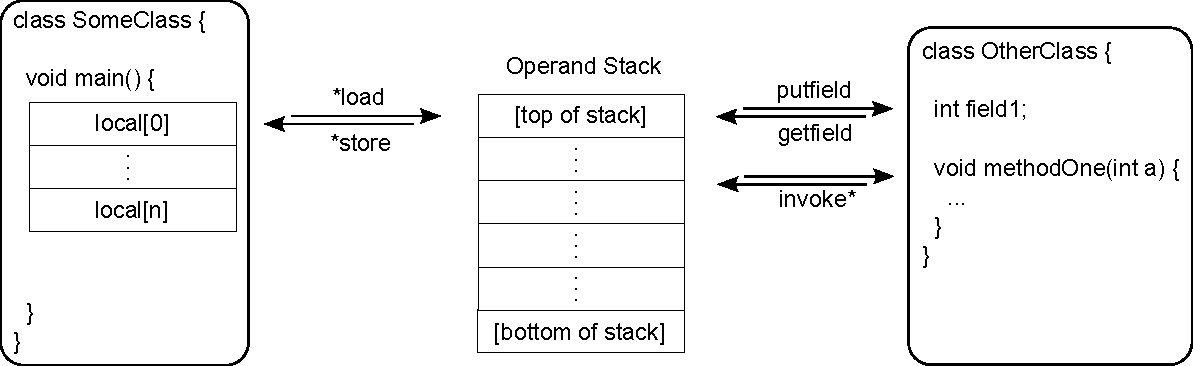
\includegraphics[width=\textwidth]{./Figures/stack-paths.pdf}
  \caption[Data Endpoints]{Data flowing through endpoints.}
	\label{fig:data-endpoints}
\end{figure}

\subsection{Operand Stack}

The \emph{operand stack} is a fixed-sized, Last In First Out (LIFO) data structure \cite[2.6.2]{jvms7} used to perform computation and store intermediary values between other data endpoints.  Each method has access to its own private operand stack during execution, the size of which is determined by the \texttt{maxStack} class file attribute that is specified at compile time.

Values are pushed onto the stack, either explicitly through load instructions or as a result of other instruction execution such as a return value being loaded to the stack after a method invocation.  Once values are on the stack, arithmetic can be performed using instructions like \texttt{iadd} and \texttt{isub} (add and subtract, respectively).  Listing \ref{operand-stack-arithmetic} shows example bytecode that loads values onto the stack and adds them.

\begin{lstlisting}[language=jvm-bytecode,caption=Operand stack arithmetic,label=operand-stack-arithmetic]
  ldc 2  // load constant 2 onto the stack
  ldc 3  // load constant 2 onto the stack
  iadd   // add the top two values on the stack
\end{lstlisting}

\subsection{Local Variables}

During execution, a method has access to a fixed number of local variable slots \cite[2.6.1]{jvms7}.  Listing \ref{locals-java} shows an example Java method that annotates how the locals array is populated.

\begin{lstlisting}[language=Java,caption=Java local variables,label=locals-java]
static int add( int b ) {  // locals[0] = b
  int i = 7;               // locals[1] = i
  int j = 6;               // locals[2] = j
  return b + i + j;
}\end{lstlisting}

Local variables are transferred to and from the operand stack with the \texttt{load} and \texttt{store} opcodes.  Figure \ref{locals-java} shows how the locals array could be allocated given local variable declarations.  Listing \ref{bc-load-store} details how the locals array would interact with the operand stack as depicted in Listing \ref{locals-java} \footnote{Note that compiler optimizations would remove the redundant loads and stores in Listing \ref{bc-load-store}, but it is instructive to retain them.}.

\begin{lstlisting}[language=jvm-bytecode,caption=Load and store,label=bc-load-store]
  ldc 7     // load the constant 7 onto the stack
  istore 1  // store 7 to locals[1]
  ldc 6     // load the constant 6 onto the stack
  istore 2  // store 6 to locals[2]
  iload 0   // load b from locals[0]
  iload 1   // load i from locals[1]
  iload 2   // load j from locals[2]
  iadd      // add i + j
  iadd      // add b to result of i + j
  iret      // return result
\end{lstlisting}

Each load instruction in Listing \ref{bc-load-store} is prefixed by an 'i' to indicate the type of value being loaded.  Integer values require an \texttt{i} prefix, while references require an \texttt{a} prefix.  

The size of the locals array is statically defined within bytecode by the \texttt{maxLocals} attribute of the method.  Attempting to access an index outside of this limit at runtime causes an exception to be thrown.

\subsection{Fields}

Field values of class instances are loaded onto the stack with the \texttt{getfield} instruction and written with the \texttt{putfield} instruction.  Listing \ref{field-java} defines a class \texttt{A} with an integer field \texttt{value} and Listing \ref{bc-getfield} shows the bytecode necessary to read from the \texttt{value} field.

\begin{lstlisting}[language=Java,caption=Java class fields,label=field-java]
package test;
class A {
  int value;
}
\end{lstlisting}

\begin{lstlisting}[language=jvm-bytecode,caption=Load the value of a field onto the stack,label=bc-getfield]
  aload [objectref:A]
  getfield test/A.value I
\end{lstlisting}

After the bytecode in Listing \ref{bc-getfield} executes, the value of the \texttt{value} field of class \texttt{A} will be on the top of the stack.  The bytecode in Listing \ref{bc-putfield} consumes the two values loaded on the stack and sets the value of the \texttt{value} field of class \texttt{A} to 7.

\begin{lstlisting}[language=jvm-bytecode,caption=Set the value of a field,label=bc-putfield]
  aload [objectref:A]
  ldc 7
  putfield test/A.value I
\end{lstlisting}

Access to static fields is performed with the \texttt{getstatic} and \texttt{putstatic} instructions, which behave identically to \texttt{getfield} and \texttt{putfield} except they do not require an object reference to be loaded onto the stack.

\subsection{Method Invocation}

Method invocation is performed by pushing arguments onto the operand stack, then using one of the invocation instructions.  Invocation instructions pop all arguments off the operand stack, including the object reference if present, and push the return value if one exists for the target method.  Each invocation instruction is referred to as a \emph{call site}, and the object reference the method is being called on is referred to as the \emph{receiver}.  Listing \ref{method-java} shows different forms of declared methods in Java source, and Figure \ref{fig:invoke-src-to-bc} shows Java invocations of those methods and the corresponding invocation bytecode.

\begin{lstlisting}[language=Java,caption=Java class methods,label=method-java]
package test;
class A {
  static int a() { ... }
  int b() { ... }
  int c(int i) { ... }
}
\end{lstlisting}

\begin{figure}[htbp]

\begin{minipage}[t]{0.45\textwidth}
\begin{lstlisting}[language=Java,frame=tlrb]
a();
obj.b();

obj.c(9);
\end{lstlisting}
\end{minipage}
\hspace{0.5cm}
\begin{minipage}[t]{0.45\textwidth}
\begin{lstlisting}[language=jvm-bytecode,frame=tlrb]
invokestatic test/A.a ()I
aload [obj]
invokevirtual test/A.b ()I
aload [obj]
ldc 9
invokevirtual test/A.c (I)I
\end{lstlisting}
\end{minipage}

\caption[Invocation Bytecode]{Mapping Java source to bytecode}
\label{fig:invoke-src-to-bc}
\end{figure}

The simplest form of invocation is a static method invocation using the \texttt{invokestatic} instruction, which requires just arguments and a symbolic link to the target method as shown on line 1 of Figure \ref{fig:invoke-src-to-bc}.  Virtual methods (methods declared without the \texttt{static} keyword), are called with the \texttt{invokevirtual} instruction, which requires the object reference of the receiver be pushed on the stack along with the arguments.  If the receiver is an interface, the \texttt{invokeinterface} instruction must be used as shown in Listings \ref{java-interface-decl} and \ref{bc-interface-invoke}.

\begin{lstlisting}[language=Java,caption=Java interface declaration,label=java-interface-decl]
package example;
interface Testable {
  void test(String s);
}
class SomeClass implements Testable {
  void test(String s) { ... }
}
\end{lstlisting}
\vspace{2em}
\begin{lstlisting}[language=jvm-bytecode,caption=Java interface invocation,label=bc-interface-invoke]
invokeinterface example/Testable test (Ljava/lang/String;)V
\end{lstlisting}

If \texttt{invokeinterface} is used with an object reference that does not implement the specified interface, a \texttt{ClassVerifyException} is thrown by the JVM at runtime.

More details about the invocation bytecode instructions can be found in Bill Venner's 1997 JavaWorld article \cite{venners-invocation}.

\section{Bytecode Verification}

All data endpoint access instructions embed not only the symbolic link to their target, but also the target's type descriptor.  Additionally, instructions generally require that a specific combination of operands with specific types are loaded onto the stack in order for them to execute without error.  After the class is loaded into memory and parsed, and before it is made available for execution to other classes within the JVM, the class is run through a verification process to statically prove each instruction has been provided its required operands in the correct order.  Any deviations from the required contract throw a \texttt{ClassVerifyException} at runtime.

\section{Generalization}

All data endpoint access discussed in this chapter goes through the same process: verify permissions, verify target type, verify operand types, and lookup receiver.  The field access instructions can be modeled as function, as shown in Table \ref{table:field-instruction-descriptors}, where \texttt{T} is the field type and \texttt{R} is the receiver type.

\begin{table}[htbp]
  \centering
  \begin{tabular}{ | l | l | p{5cm} |}
  \hline
  \textbf{Instruction} & \textbf{Descriptor} \\ \hline
  \texttt{getfield} & \texttt{(R)T} \\ \hline
  \texttt{putfield} & \texttt{(R,T)V} \\ \hline
  \texttt{getstatic} & \texttt{()T} \\ \hline
  \texttt{putstatic} & \texttt{(T)V} \\ \hline
  \end{tabular}
  \caption[Field Instruction Descriptors]{Field instructions modeled as functions.}
  \label{table:field-instruction-descriptors}
\end{table}

With all data endpoint JVM instructions generalized to function invocations, instructions can be composed at runtime, as Chapter \ref{chapter:Invokedynamic} will discuss in detail.






\chapter{Invokedynamic}
\label{chapter:Invokedynamic}
\lhead{ \leftmark }

Though non-Java languages have been running on the JVM since its initial public release, no real effort was made by the engineers within Sun (now Oracle) to make the JVM a hospitable host to languages with semantics that differed from Java.  As more production languages (such as JRuby) used JVM-based runtimes, it became apparent to Sun that more work needed to be done at the JVM level to support these languages.  The goal was to make the JVM more flexible and adaptable while still retaining the strong type verification required to enforce Java's type system.  In order to accomplish this, fundamental changes to the JVM were needed.  These modifications to core JVM functionality, a so-called "renaissance" of the JVM, were created as a branch of the OpenJDK project named the \emph{Da Vinci Machine Project} in mid-2006 and formalized under JSR-292 \cite{jsr-292}.  The finalized implementation was included in the release of JDK 7.  The modifications included low cost function pointers in the form of method handles, new method linking options with the \texttt{invokedynamic} instruction, and changes to the runtime optimizer.

\section{Method Handles}

Before JSR-292, the smallest composable unit within the JVM was the class.  The only available facility to pass invokable references to methods was the Core Reflection API, which was not designed for performance intensive applications.  The Core Reflection API was designed as a meta layer to provide introspection to classes and their declared fields and methods at runtime.  The runtime support for Reflection existed outside of the reach of the JVM optimizer, which meant that reflective invocations could not benefit from optimization heuristics such as inlining \cite{jrose-methodhandles}.  Reflective invocations performed access control checks at each invocation, which resulted in significant overhead at runtime \cite{vmil09}.  Instead of attempting to redefine the behavior of the Core Reflection API and break backwards compatibility, the JSR-292 Expert Group elected to create a new abstraction.  Instead of separate classes to model fields and methods like the existing Core Reflection API, a single interface was created to abstract both field modification and method invocation bytecode instructions: the method handle.

Method handles are function pointers represented as a method descriptor that encapsulate field modification and method invocation operations.  They are represented in the Java standard library in JDK 7 by the \texttt{MethodHandle} class in the \texttt{java.lang.invoke} package.  Unlike the Core Reflection \texttt{Field} and \texttt{Method} classes, a method handle does not exist to provide metadata or perform runtime introspection.  A method handle is meant purely as an efficient means of invoking a functional representation of a bytecode instruction.  Listing \ref{indy-targets-java} defines a class, \texttt{A} with a single field and three methods that are resolved using a \texttt{MethodHandles.Lookup} in Listing \ref{acquire-method-handles}.

\begin{lstlisting}[language=Java,caption=Java field and method lookup targets,label=indy-targets-java]
package test;
class A {
  int value;
  static int a() { ... }
  int b() { ... }
  int c(boolean x) { ... }
}
\end{lstlisting}
\vspace{4em}
\begin{lstlisting}[language=Java,caption=Reflective lookup using \texttt{MethodHandles.Lookup},label=acquire-method-handles]
MethodHandles.Lookup lookup = MethodHandles.lookup();
MethodHandle mh1 = lookup.findGetter(A.class, "value",
                          methodType(int.class));
MethodHandle mh2 = lookup.findStatic(A.class, "a",
                          methodType(int.class));
MethodHandle mh3 = lookup.findVirtual(A.class, "b",
                          methodType(int.class));
MethodHandle mh4 = lookup.findVirtual(A.class, "c",
                          methodType(int.class, boolean.class));
\end{lstlisting}

The descriptors of the method handles acquired in Listing \ref{acquire-method-handles} are listed in Table \ref{table:acquire-method-handles-descriptors}.

\begin{table}[htbp]
  \centering
  \begin{tabular}{ | l | l | p{5cm} |}
  \hline
  \textbf{Method Handle} & \textbf{Descriptor} \\ \hline
  mh1 & \texttt{(Ltest/A;)I} \\ \hline
  mh2 & \texttt{()I} \\ \hline
  mh3 & \texttt{(Ltest/A;)I} \\ \hline
  mh4 & \texttt{(Ltest/A;Z)I} \\ \hline
  \end{tabular}
  \caption[Method Handle Descriptors]{The descriptors of the method handles acquired in Listing \ref{acquire-method-handles}.}
  \label{table:acquire-method-handles-descriptors}
\end{table}

Each \texttt{MethodHandle} can then be called using its \texttt{invoke(Object...)} method, which performs the underlying field access or method invocation.

\section{Method Handle Combinators}

Now that the previously disjoint operations are unified with a common functional abstraction, they can be combined into composite operations.  The potential of method handles is to generate and reconfigure code at runtime without generating and loading raw bytecode into a class loader.  Instead, method handles can be composed with one another -- a function pointer that calls another function pointer -- and integrated with existing class methods to allow flexible code structures constructed solely from method handles that the native code optimizer within the JVM is aware of and able to optimize.

Every bytecode instruction involving data endpoints is representable as a method handle.  These baseline method handles are provided by the \texttt{MethodHandles} class included in the \texttt{java.lang.invoke} package in JDK 7.  The \texttt{MethodHandles} class provides method handles that filter arguments and return values, spread and collect vararg arguments, and conditionally branch between method handles.

\subsection{Filters}
\label{section:filters}

The \texttt{filterArguments()} and \texttt{filterReturnValue()} in the \texttt{MethodHandles} class enable method handles to be adapted to call site descriptors or linked together.  For example, given the classes \texttt{A}, \texttt{B}, and \texttt{C} in Listing \ref{pointer-classes}, evaluating the expression \texttt{a.b.c.value} would require the bytecode listed in Listing \ref{nested-get-bytecode}.

\begin{lstlisting}[language=Java,caption=Classes to execute \texttt{getfield} instructions against,label=pointer-classes]
  class A {
    B b;
  }
  class B {
    C c;
  }
  class C {
    int value;
  }
\end{lstlisting}
\vspace{2em}
\begin{lstlisting}[language=jvm-bytecode,caption=Nested property accessor bytecode,label=nested-get-bytecode]
  aload [a]
  getfield A.b
  getfield B.c
  getfield C.value
\end{lstlisting}

This behavior can now be encapsulated into a single method handle by composing multiple method handles and filtering their return values.  Table \ref{table:method-handle-descriptor-equations} lists equations that describe each method handle performing getfield operations for \texttt{a.b.c.value}.

\begin{table}[htbp]
  \centering
  \begin{tabular}{ | l | l | p{5cm} |}
  \hline
  \textbf{Bytecode Operation} & \textbf{Equation} \\ \hline
  \texttt{getfield A.b} & ${m^{d}}_0 = (A) \to B$ \\ \hline
  \texttt{getfield B.c} & ${m^{d}}_1 = (B) \to C$ \\ \hline
  \texttt{getfield C.value} & ${m^{d}}_2 = (C) \to I$ \\ \hline
  \end{tabular}
  \caption[\texttt{getfield} Descriptors]{Equation representation of the method handle descriptors.}
  \label{table:method-handle-descriptor-equations}
\end{table}

The return value of each method handle is then filtered through the next method handle in the chain:
\[ {m^{d}}_0(A) \to {m^{d}}_1(B) \qquad
   {m^{d}}_1(B) \to {m^{d}}_2(C) \qquad
   {m^{d}}_2(C) \to I \]
After substitution, the method handle tree simplifies down to a method handle that takes an argument of type \texttt{A} and returns the \texttt{int} value of the \texttt{value} field in class \texttt{C}: $\quad{m^{d}}_0(A) \to I  $.

A visual representation of this filtering process is depicted in Figure \ref{fig:pointer-getfield}.

\smallskip
\begin{figure}[htbp]
  \centering
    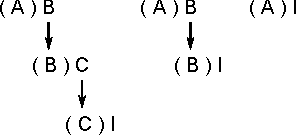
\includegraphics{./Figures/pointer-getfield.pdf}
  \caption[Method Handle Composition]{A tree of method handles simplify through substitution.}
	\label{fig:pointer-getfield}
\end{figure}

Filtering allows one complex operation to be wrapped into one method handle that can then be invoked, passed as a single object reference to other code, or composed with other method handles for even more complex behavior.

\subsection{Spreaders and Collectors}

A method handle with the descriptor \texttt{(A,B,C)D} could be adapted to a more general method handle with the descriptor \texttt{(Object[])Object} using the \texttt{asVarArgsCollector(Object[].class)} method of the \texttt{MethodHandle} class.  This collects the arguments \texttt{A}, \texttt{B}, and \texttt{C} into the \texttt{Object[]} argument of the adapted method handle.  The inverse operation can be performed with the \texttt{asSpreader(Class<?>, int)} method of the \texttt{MethodHandle} class, which takes all arguments from the provided integer offset and "spreads" them -- distributes them as individual parameters -- back to the original \texttt{(A,B,C)D} form.

\subsection{Guards}

Guards enable the composition of a traditional if-then-else statement using method handles.  Constructing a guard is done by the \texttt{guardWithTest} method within the \texttt{MethodHandles} class which requires three method handles as arguments.  First, a guard predicate which returns a \texttt{boolean} type.  Second, a target method handle to invoke if the guard predicate is true.  Third, a fallback method handle to invoke if the guard predicate is false.  Using another guard as the fallback method handle enables the construction of a tree of conditional branches.

\section{Invocation Linking}

The inflexibility of the JVM prior to JDK 7 stems from the rigidity of the invocation instructions.  The modifications implemented in the Da Vinci Machine Project that make this linkage process more flexible come in the form of a new invocation instruction, \texttt{invokedynamic}.

\subsection{\texttt{invokevirtual} Invocation}

As detailed in Chapter \ref{chapter:JVM}, the JVM uses an internal symbolic linking process to link an invocation instruction, a \emph{callsite}, to the target class method.  During this process the type descriptor embedded in the call site is compared to the type descriptor of the target method and an exception is thrown by the JVM if the type descriptors are not compatible.  A depiction of the linking process for the invocation instruction in Listing \ref{java-normal-invoke-bytecode} is shown in Figure \ref{fig:linking-invokevirtual}.
\vspace{2em}
\begin{lstlisting}[language=jvm-bytecode,caption=virtual method invocation bytecode,label=java-normal-invoke-bytecode]
invokevirtual path/to/OtherClass.otherMethod (I)V
\end{lstlisting}
\vspace{2em}
\begin{figure}[htbp]
	\centering
		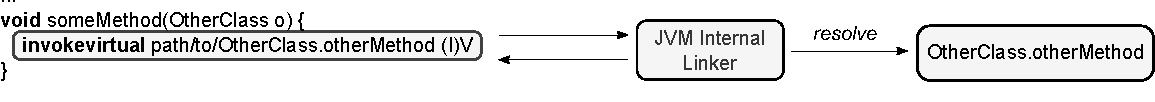
\includegraphics[width=\textwidth]{./Figures/linking-invokevirtual.pdf}
	\caption[invokevirtual Linking]{JVM runtime internally resolves symbolic link.}
	\label{fig:linking-invokevirtual}
\end{figure}

\subsection{\texttt{invokedynamic} Invocation}

Instead of a hardwired symbolic link to the target method, \texttt{invokedynamic} call sites embed a symbolic link to a static \emph{bootstrap} method which returns a \texttt{CallSite} object.  The \texttt{CallSite} object contains a \texttt{MethodHandle} which points to the invocation target method.  Simply put, instead of specifying a target method, an \texttt{invokedynamic} call site specifies "who to ask" to get a target method.  Along with the bootstrap method symbolic link, \texttt{invokedynamic} call sites also embed the target method name and type descriptor, which acts as a contract that must be fulfilled by the method handle in the call site returned by the bootstrap method.  An example \texttt{invokedynamic} instruction and corresponding linkage visualization are depicted in Listing \ref{java-indy-invoke-bytecode} and Figure \ref{fig:linking-invokedynamic}, respectively.
\vspace{2em}
\begin{figure}[htbp]
	\centering
    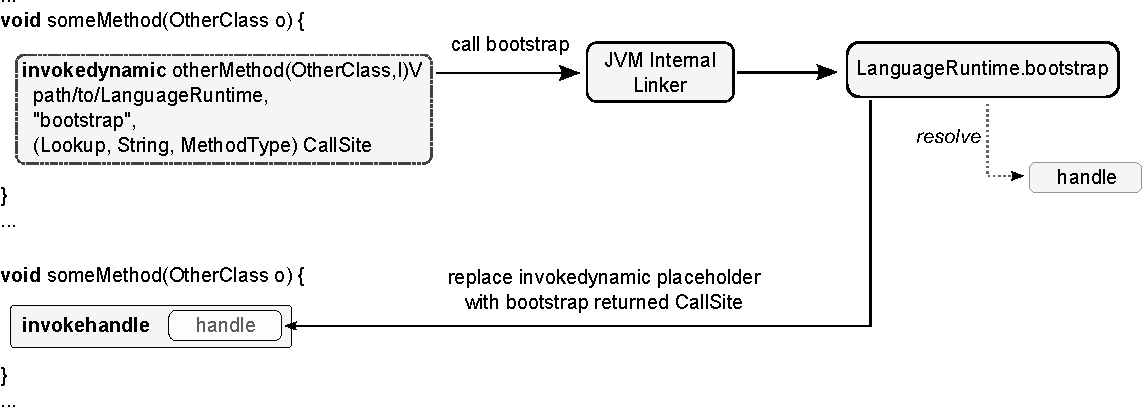
\includegraphics[width=\textwidth]{./Figures/linking-indy-bootstrap.pdf}
	\caption[invokedynamic Linking]{JVM runtime defers to user code bootstrap to resolve symbolic link.}
  \label{fig:linking-invokedynamic}
\end{figure}
\vspace{2em}
\begin{lstlisting}[language=jvm-bytecode,caption=dynamic invocation bytecode,label=java-indy-invoke-bytecode]
invokedynamic
  otherMethod(OtherClass,I)V           // signature being invoked
  path/to/LanguageRuntime.bootstrap    // CallSite provider
  (Lookup, String, MethodType)CallSite // bootstrap signature
\end{lstlisting}

The bootstrap method uses the reflective \texttt{MethodHandle.Lookup} class to obtain method handles, and can optionally perform any combination of method handle adaptation as discussed in Section \ref{section:filters}.  The bootstrap method is defined in JVM bytecode just like any other class, as opposed to the internal JVM process that links the other invocation instructions.  Listing \ref{indy-bootstrap-example} defines an example bootstrap method.

\begin{lstlisting}[language=Java,caption=A bootstrap method,label=indy-bootstrap-example]
class LanguageRuntime {
  static CallSite bootstrap( Lookup lookup,
                             String methodName,
                             MethodType type ) {
    MethodHandle mh = // resolve a MethodHandle ...
    return new MutableCallSite(mh);
  }
}
\end{lstlisting}

\subsection{Call Site Relinking}

\texttt{CallSite} is an abstract base class extended by \texttt{ConstantCallSite} and \texttt{MutableCallSite}.  A \texttt{ConstantCallSite} cannot be re-targeted to another method handle, while the \texttt{MutableCallSite} can be updated with its \texttt{setTarget(MethodHandle)} method.  A \texttt{ConstantCallSite} generally has better performance at the price of flexibility, but the \texttt{MutableCallSite} is useful in building adaptive call sites that are able to rebuild themselves in response to the receivers invoked on them.

\subsection{Optimization}

The primary feature that sets method handles and the \texttt{invokedynamic} infrastructure apart from other JVM features like the Core Reflection API is that method handles are designed to be able to take advantage of many of the optimizations applied to normal bytecode \cite{direct-method-handles}.  Specifically, method handles can be inlined and constant folded as the method handle tree symbols are evaluated and optimized at runtime.



\chapter{Structural Typing}
\label{chapter:StructuralTyping}
\lhead{ \leftmark }

A type system that requires equivalent types to have the same declared name, regardless of whether they define identical fields and methods, is referred to as a \emph{nominal} (or \emph{nominative}) type system.  A type system that ignores the declared name of types and only requires equivalent types to share common field or method declarations is referred to as a \emph{structural} type system.  More formally, for types $T_0$ and $T_1$, in a nominal type system $T_0 \equiv T_1 \iff {T_0}_{name} = {T_1}_{name}$. In a structural type system $T_0 \equiv T_1 \iff \forall \; F \in {T_0}_{SLOTS} \; \exists \; F' \in {T_1}_{SLOTS}, F_{TYPE} \equiv {F'}_{TYPE} $ where slots can be a field or method defined within the given type.

\section{Nominal Typing}

As described in chapter \ref{chapter:JVM}, the JVM uses nominal types throughout.  Type names are declared in Java source, embedded into bytecode instructions, and enforced at runtime by the JVM.  As shown in Listing \ref{types-nominal}, even though classes \texttt{A} and \texttt{B} are structurally identical, they are not considered equivalent within Java or by the JVM at runtime, and therefore cannot be used interchangeably.

\begin{lstlisting}[language=Java,caption=Nominal types,label=types-nominal]
  class A {
    void test() { ... }
  }
  class B {
    void test() { ... }
  }
  void m1(A a) {
    a.test();
    m2(a);      // illegal
  }
  void m2(B b) {
    b.test();
    m1(b);      // illegal
  }
\end{lstlisting}


\subsection{Case Study: java.io.Closeable}

Prior to the release of J2SE 1.5 in 2004, the Java standard library developers noticed they had several classes in the \texttt{java.io} package that all had \texttt{close()} methods.  They wanted to be able to write generalized code that could operate on all of these classes, but the classes all had different hierarchies -- they extended different base classes -- so they could not be addressed as one common type.  To solve this problem, the \texttt{java.io.Closeable} interface was introduced.  This interface defines only a \texttt{close()} method that throws an \texttt{IOException}, and is meant to enables objects that represented resources such as files and network connections to be closed without the caller knowing anything about the class implementation other than the fact that it implements \texttt{close()}.

However, this presented a problem when dealing with the large collections of code already written.  Existing classes that had \texttt{close()} methods but did not explicitly implement the \texttt{Closeable} interface -- because it didn't exist when the code was written -- could not be passed as an argument to code expecting an instance of \texttt{Closeable}.  Due to Java's nominal type system, existing code would have to be modified to add the \texttt{implements Closeable} declaration to every relevant class definition and then be recompiled and released as a new version.

One solution to the \texttt{Closeable} problem would be to create a way for classes that do not explicitly implement the \texttt{Closeable} interface to still be treated as equivalent to the \texttt{Closeable} interface as long as they implement that single \texttt{close()} method.  That concept is a form of structural typing.

\section{Structural Typing}

Listing \ref{types-structural} demonstrates both the benefits and potential pitfalls of structural typing.  Similar to Listing \ref{types-nominal}, two structurally equivalent types are defined.  The difference is that, since \texttt{Cowboy} and \texttt{Rectangle} are structurally identical and they are defined within a structural type system, they can be used interchangeably on lines 9 and 13.

\begin{lstlisting}[language=Java,caption=Structural types,label=types-structural]
  class Cowboy {
    void draw() { ... }
  }
  class Rectangle {
    void draw() { ... }
  }
  void drawGun(Cowboy cowboy) {
    cowboy.draw();
    paint(cowboy);      // legal
  }
  void paint(Rectangle rect) {
    rect.draw();
    drawGun(rect);      // legal
  }
\end{lstlisting}

This approach solves the \texttt{java.io.Closeable} problem.  Code could be written within this system that operated on both the \texttt{Cowboy} and \texttt{Rectangle} types uniformly, even though they have no explicitly declared relation to one another.  New interfaces can be written that existing classes implicitly implement without modification.  However, this interchangeable usage should immediately be cause for concern.  The \texttt{draw()} method in Listing \ref{types-structural}, while lexically identical in each class, has a different meaning within the domain of each class.  In the context of a \texttt{Cowboy}, to \texttt{draw()} means to draw a gun.  In the context of a \texttt{Rectangle}, \texttt{draw()} means to render itself.  This is an example of the ambiguity of the English language leaking into what should be a more formal definition within a programming language.  This \emph{accidental equivalence}, an edge case within structural type systems, can be mitigated through a hybrid use of structural typing with \emph{structural interfaces}.

\subsection{Structural Interfaces}

There is a design compromise between structural typing and nominal typing that solves the \texttt{java.io.Closeable} problem while minimizing accidental equivalence.  Described with Java-like syntax in Listing \ref{types-structural-interfaces}, the hybrid approach uses nominal typing to determine equivalence of two classes and structural typing to determine whether a type conforms to an interface.

\begin{lstlisting}[language=Java,caption=Structural interface,label=types-structural-interfaces]
  class Cowboy {
    void draw() { ... }
    int getHeight() { ... }
  }
  class Rectangle {
    void draw() { ... }
    int getHeight() { ... }
  }
  interface Height {
    int getHeight();
  }
\end{lstlisting}

In Listing \ref{types-structural-interfaces}, \texttt{Cowboy} and \texttt{Rectangle} both conform to the \texttt{Height} interface by implementing the \texttt{getHeight()} method and can be provided to any receiver that is expecting an instance of \texttt{Height}.  However, even though \texttt{Cowboy} and \texttt{Rectangle} have identical structures they are not equivalent to each other and cannot be used interchangeably, thereby limiting accidental equivalence errors.

\section{Implementation}

The implementation challenges of structural interfaces stem from the fact that each concrete type (a type that corresponds to a specific memory layout) has the potential to implicitly implement a large number of interfaces.  An interface like \texttt{java.io.Closeable} in a structural type system could be implemented by hundreds of concrete types, so when a function accepts an instance of \texttt{java.io.Closeable} as a parameter and calls its \texttt{close()} method the compiler has no idea which of the hundreds of implementing types will be passed to the function at runtime.  If the fields and methods of a concrete type are generalized as \emph{slots} (an offset within the memory layout of the concrete type), the problem can be described as whether the compiler can calculate the offset of a slot based only on information available at the call site at compile time, or if the offset of the slot cannot be determined until runtime.

\subsection{Compile-Time Slot Lookup}

Each name of a class in Java corresponds to one and only one memory layout of the fields and methods of that class.  Listing \ref{code-layout-nominal} defines several Java classes, and Figure \ref{fig:memory-layout-nominal} shows an approximation of the corresponding memory layout.

\begin{lstlisting}[language=Java,caption=Nominal type inheritance,label=code-layout-nominal]
  class Base {
    void sayHello() { ... }
  }
  class Class1 extends Base {
    void m1() { ... }
    void sayHello() { ... }
  }
  class Class2 extends Base {
    void m2() { ... }
    void sayHello() { ... }
    void m3() { ... }
  }
  class Class3 extends Class2 {
    void m2() { ... }
    void sayHello() { ... }
    void m4() { ... }
  }
\end{lstlisting}

\begin{figure}[htbp]
  \centering
    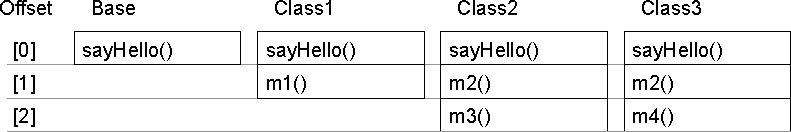
\includegraphics[width=\textwidth]{./Figures/memory-layout-nominal.pdf}
  \caption[Single Inheritance Memory Layout]{An abstract representation of class memory layout.}
	\label{fig:memory-layout-nominal}
\end{figure}

Given a pointer to an instance of \texttt{Base}, the compiler knows at compile time that \texttt{sayHello()} will always be located at offset \texttt{[0]}.  The same relationship exists between \texttt{Class2} and its subclass, \texttt{Class3}.  Given a pointer to any class that extends \texttt{Class2}, \texttt{m2()} will always be at offset \texttt{[1]}.  Each subclass aligns its lower offsets with its base class structure, then uses its higher offsets for its own structure.  This predictability enables a compiler to calculate the offset of any field or method of a class and generate a simple indirect load or jump instruction to access it.

\subsection{Runtime Slot Lookup}

Listing \ref{code-layout-structural} shows pseudocode of two interfaces and two classes.  \texttt{Class1} and \texttt{Class2} both implement the \texttt{Stream} interface by implementing \texttt{close()}.  \texttt{Class2} also implements the \texttt{Gettable} interface by implementing \texttt{get()}.

\begin{lstlisting}[language=Java,caption=Pseudocode: Java with structural types,label=code-layout-structural]
  interface Gettable {
    void get();
  }
  interface Stream {
    void close();
  }
  class Class1 {
    void close() { ... }
  }
  class Class2 {
    void close() { ... }
    void get() { ... }
  }
  void call( Stream stream ) {
    stream.close();
  }
\end{lstlisting}

\begin{figure}[htbp]
  \centering
    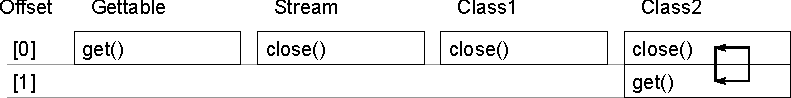
\includegraphics[width=\textwidth]{./Figures/memory-layout-structural.pdf}
  \caption[Structural Inheritance Layout]{An abstract representation of class memory layout.}
	\label{fig:memory-layout-structural}
\end{figure}

When calling into concrete types, the offset of a given method was known at compile time.  With structural typing this is no longer the case, as evident by the memory layout of \texttt{Class2} in Figure \ref{fig:memory-layout-structural}.  Since \texttt{Class2} implements both the \texttt{Gettable} and \texttt{Stream} interfaces it must allocate a slot in its memory layout for both the \texttt{get()} and \texttt{close()} methods.  However, both of those methods are defined at offset \texttt{[0]} in their respective interfaces.  If a compiler places the \texttt{close()} method at offset \texttt{[0]} of \texttt{Class2}, any call sites receiving an instance of \texttt{Class2} as a \texttt{Gettable} cannot predict at compile time the offset at which the \texttt{get()} method will be located.  The inverse is also true if the \texttt{get()} method was placed at offset \texttt{[0]}.  This problem is aggravated when more than two interfaces are considered across multiple concrete types.

The offset that must be resolved on the receiver from the call site on line 15 cannot be determined through static analysis.  The call site could be provided either \texttt{Class1} or \texttt{Class2} at runtime, and must be able to efficiently lookup the offset for the \texttt{close()} method on that type and invoke it.  This ad-hoc type introspection requirement has the potential to introduce significant overhead per invocation.

Prior to \texttt{invokedynamic}, the rigid nature of the invocation bytecode instructions meant the options to lookup and call methods on types at runtime were limited.  Implementing a feature like structural typing on the JVM required either reflection or a code generation technique that generated inline type checks at the call site at compile time \cite{structural-types-scala}.  Neither option was preferable, since reflection introduced significant overhead and the code generation technique cannot account for types that are unknown at compile time.

With \texttt{invokedynamic} method lookup overhead can be reduced by having the call site itself cache references to methods by receiver type as they are invoked.  This approach has the potential to completely eliminate the method lookup as long as the receiver type is in the call site cache.

\section{Inline Caching}

An \emph{inline cache} is a dispatch table embedded in a call site that builds an associative cache of receiver type metadata in order to optimize future invocations.  Inline caching was first developed for use in Smalltalk implementations in the 1980s \cite{smalltalk-pic} in order to improve dynamic invocation performance.  Listing \ref{code-interface-callsite} defines an interface call site that could benefit from inline caching.

\begin{lstlisting}[language=Java,caption=An interface call site,label=code-interface-callsite]
  interface Gettable {
    void get();
  }
  class A {
    void get() { ... }
  }
  class B {
    void get() { ... }
  }
  class C {
    void get() { ... }
  }
  void call( Gettable g ) {
    g.get();
  }
\end{lstlisting}

On the first invocation of \texttt{call(Gettable)} in Listing \ref{code-interface-callsite}, the inline cache of call site \texttt{g.get()} will be empty.  If, for example, an instance of class \texttt{A} was passed as the parameter on the first invocation, a full lookup would have to be performed to examine the methods implemented in class \texttt{A} and find \texttt{get(Greetable)}.  Once it is resolved, however, the offset of \texttt{get()} within class \texttt{A} will be added to the inline cache as an association between the receiver type \texttt{A} and the method handle of \texttt{get()} within type \texttt{A}.

Depending on how many receivers a call site is associated with, it can be referred to as either \emph{monomorphic}, \emph{polymorphic}, or \emph{megamorphic}.
 
\subsection{Monomorphic}

According to research by Oracle's HotSpot engineering team, 90\% of call sites only target one concrete method over their entire lifetime \cite{hotspot-virtualcalls}.  These call sites, called \emph{monomorphic}, retain a reference to the previously invoked receiver type.  Upon subsequent invocation, the previous receiver type is compared to the new receiver type and, if they match, the cached receiver metadata can be used to jump directly to the target method.

The design decisions inherent to monomorphic call sites all revolve around the caching heuristics.  Primarily, what happens on a cache miss?  If a call site replaces its cached receiver type each time the new receiver doesn't match, the overhead of cache maintenance could dominate execution time if a call site is being called with two types in an alternating invocation pattern.  Conversely, choosing to not replace the cached receiver type could miss an optimization opportunity.  One approach to avoid these issues, developed as an extension to the monomorphic inline cache by Sun Microsystems for the Self project, is to simply grow the cache to accommodate new receiver types \cite{self-pic}.

\subsection{Polymorphic}

A \emph{polymorphic inline cache} is an inline cache that stores multiple receiver types.  Pseudocode for a polymorphic inline cache for the call site in Listing \ref{code-interface-callsite} is demonstrated in Algorithm \ref{algo:poly-cache}.

\begin{flushright}
\begin{algorithm}[H]
 \SetAlgoLined
 \Switch{ receiver.type }{
  \lCase{A}{ A.get()\; }
  \lCase{B}{ B.get()\; }
  \lCase{C}{ C.get()\; }
  \lOther{
    lookup(receiver)\;
  }
 }
 \label{algo:poly-cache}
 \caption{Inline cache method dispatch}
\end{algorithm}
\end{flushright}

\smallskip

For the roughly 10\% of call sites that are invoked against more than one receiver type, a polymorphic inline cache is allocated with initial space to store several receiver types.  If a new receiver type is used at the call site, it falls through to the slower \texttt{lookup()} function which performs a linear search on the receiver type for the target method, then adds it to the cache.

This behavior can be implemented with a tree of method handles as depicted in Figure \ref{fig:guard-pic}.

\begin{figure}[htbp]
	\centering
    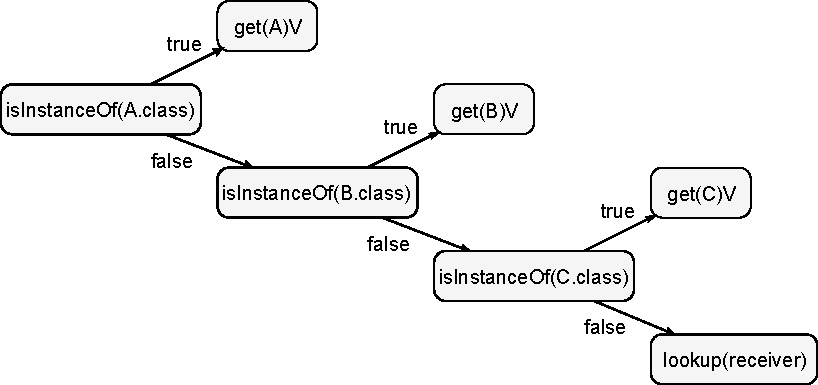
\includegraphics[width=\textwidth]{./Figures/guard-pic.pdf}
	\caption[Method Handle PIC]{A polymorphic inline cache implemented with nested method handles.}
  \label{fig:guard-pic}
\end{figure}

Constructed with the \texttt{guardWithTest()} factory method in the \texttt{MethodHandles} class, the guard is bound to the \texttt{isInstanceOf(Class)} method of the \texttt{java.lang.Class} metaclass of the receiver.  If the guard succeeds, it immediately invokes a method handle that references the concrete method.  If the guard fails, the fallback of the guard is the guard of the next receiver type check.  There are several optimization variations that influence how this tree can be constructed.  New types can be added to the root of the tree or inserted before the final \texttt{lookup(receiver)} call.  Invocation counts could be tracked, bubbling up the most invoked receiver type to the root of the tree so it is checked first in order to speed up dispatch time.  However, obviously the tree cannot grow without bound.  The inline cache must be designed to handle the 1\% of cases where an unmanageable number of types flow through one call site.

\subsection{Megamorphic}

A call site that handles an inordinate amount of receiver types is referred to as \emph{megamorphic}.  In this state efficient polymorphic dispatch is not possible, since too much time would be consumed walking the cache entries and comparing them to the new receiver.  Megamorphic call sites often revert back to an unoptimized vtable-based dispatch mechanism  \cite{hotspot-compiledcall}.


\chapter{Kale Language}
\label{chapter:Kale}
\lhead{ \leftmark }

\section{Overview}

Kale is a strongly typed programming language with structural interfaces that has been designed to prototype structural typing on the JVM using \texttt{invokedynamic}.  Many design elements of Kale are inspired by the Google Go \cite{golang-spec} programming language.

\subsection{Types}

Types declarations in Kale are analogous to classes in Java.  Types can be declared with zero or more fields and methods, all of which are annotated with type names.  Listings \ref{javaClass1} and \ref{kaleType1} show how Java syntax maps to Kale syntax.

\begin{minipage}[t]{0.45\textwidth}
\begin{lstlisting}[language=Java,caption=A Java code example,label=javaClass1]
  package test;
  class Person {
    int age;
    String name;
    String getName() {
      return this.name;
    }
  }
\end{lstlisting}
\end{minipage}
\hspace{0.5cm}
\begin{minipage}[t]{0.45\textwidth}
\begin{lstlisting}[language=Kale,caption=A Kale code example,label=kaleType1]
  package test
  type Person {
    age int;
    name string;
    getName() string {
      return this.name;
    }
  }
\end{lstlisting}
\end{minipage}

Kale using trailing type annotations instead of the leading type annotations of most C-derived languages.  Google Go's development team found this allows more complex declarations to be read left to right \cite{golang-decl-syntax} instead of the "spiral pattern" of C \cite{c-spiral-decl}.  Regardless of the small syntactical differences, both Listing \ref{javaClass1} and \ref{kaleType1} compile down to the same bytecode.

\begin{wrapfigure}{R}{0.4\textwidth}
\begin{lstlisting}[language=Kale,caption=A Kale interface,label=kaleInterface1]
  package test
  interface A {
    a();
  }
  type T {
    a() { }
  }
\end{lstlisting}
\end{wrapfigure}

Structurally typed interfaces are declared with the \texttt{interface} keyword and can only contain method declarations  -- no method bodies.  Listing \ref{kaleInterface1} defines an interface \texttt{A} that is implemented by type \texttt{T}.  Note that if the return type of a method is omitted, \texttt{void} is assumed.

\begin{wrapfigure}{R}{0.4\textwidth}
\begin{lstlisting}[language=Kale,caption=A Kale main function,label=kaleFunctions1]
  package test
  main() {
    
  }
\end{lstlisting}
\end{wrapfigure}

Kale, unlike Java, allows functions to be declared outside the scope of a class.  Listing \ref{kaleFunctions1} shows a legal Kale program with only a main function declared.

\subsection{Operators}

Kale implements a simplified version of operator overloading.  Listing \ref{kaleOperators1} demonstrates a \texttt{Vector} type that has a \texttt{+} operator.

\begin{lstlisting}[language=Kale,caption=Operators in Kale,label=kaleOperators1]
  package test
  type Vector {
    x int;
    y int;
    z int;
    + operator(v1 Vector, v2 Vector) Vector {
      v = Vector();
      v.x = v1.x + v2.x;
      v.y = v1.y + v2.y;
      v.z = v1.z + v2.z;
      return v;
    }
  }
\end{lstlisting}

Operators are made possible by Kale's relaxed tokenization rules.  The only special lexeme types are control characters like parentheses, braces, and brackets, or punctuation like semi-colons, commas, and full stops.  All other lexemes, even arithmetic operators, are considered symbols.  Operators are detected in the parser by an occurrence of three consecutive symbols, in which case the first and third symbols are considered the operands and the second symbol is considered the operator.  Usage of the operator defined in Listing \ref{kaleOperators1} is shown in Listing \ref{kaleOperatorsUse}.

\begin{wrapfigure}{R}{0.4\textwidth}
\begin{lstlisting}[language=Kale,caption=Operator use in Kale,label=kaleOperatorsUse]
  v1 = Vector();
  v1.x = 2;
  v2 = Vector();
  v2.x = 3;
  
  v3 = v1 + v2;
  // assert v3.x == 5
\end{lstlisting}
\end{wrapfigure}

Operator invocation is constructed as a chain of function invocations, so another way of writing \texttt{v1 + v2} would be \texttt{v1.+(v2)} and \texttt{v1 + v2 + v3} would be \texttt{v1.+(v2).+(v3)}.  Parentheses can alter evaluation order, turning \texttt{v1 + (v2 + v3)} into \texttt{v1.+(v2.+(v3))}.

This ignores the usual order of operations for basic arithmetic, but makes reasoning about operator use in complex types like a \texttt{Vector} or \texttt{Point} more straightforward.

\begin{comment}
\subsection{Pointers}

\begin{lstlisting}[language=Kale,caption=Pointers in Kale,label=kalePointers1]
  package test
  type Person {
    name string;
    getName() string {
      return this.name;
    }
  }
  extractName( p Person ) string {
    return p.name;
  }
  main() {
    person = Person();
    person.name = "John";
    extractName( &(person) ); // returns "John"
    &(person.name);           // pointer to "John"
    &(person.getName);        // MethodHandle (Person)Ljava/lang/String;
  }
\end{lstlisting}

With garbage collection, stack vs heap allocation is not an issue.  A pointer can safely be passed to external code



\subsection{Control Structures}

if/else

while

\end{comment}

\section{Compilation}

The Kale compiler accepts Kale source and generates JVM bytecode as output.  The compiler is implemented in Java and uses a custom lexer and recursive descent parser to build an abstract syntax tree (AST).  JVM bytecode is emitted directly from the AST through calls to the ASM bytecode generation library \cite{asm-library}, and can be loaded directly into a \texttt{ClassLoader} and executed or packaged into a jar file.

Since Kale programs differ slightly from Java in structure and content, some conversions must be applied in order to map Kale programs to class files.  First, since Kale allows a broader range of characters in symbols compared to Java, symbols used for class and method names must be converted to an equivalent \emph{unqualified name} as defined by the JVM specification \cite[4.2.2]{jvms7}.  Additionally, functions defined outside the scope of a class within a package must be packaged inside of a class.  For this reason, a \texttt{\_\_functions} class is generated within the declared package that contains all package-level functions.

\subsection{Invocations}

Since Kale uses a mix of concrete types and structural interfaces, invocations generate a mix of \texttt{invokevirtual} and \texttt{invokedynamic} instructions.  Listing \ref{kaleInvocations1} defines an interface, \texttt{Gettable}, and a type that implements that interface, \texttt{Stream}.  In the \texttt{main()} function a new instance of \texttt{Stream} is created, and passed as a parameter to \texttt{callGet(Gettable)}.  The invocation \texttt{g.get()} generates an \texttt{invokedynamic} call site, since it is being invoked against an interface.  All other invocations, including the call to \texttt{internal()} within the \texttt{Stream} class, use an \texttt{invokevirtual} instruction.

\begin{lstlisting}[language=Kale,caption=Invocations in Kale,label=kaleInvocations1]
package some.test
interface Gettable {
  get();
}
type Stream {
  get() {
    internal();
  }
  internal() {
    // no-op
  }
}
callGet( g Gettable ) {
  g.get();
}
main() {
  s = Stream();
  callGet(s);
}
\end{lstlisting}

It is very tempting to simply replace every invocation with an \texttt{invokedynamic} instruction to simplify the code generation and allow for maximum flexibility.  However, while the \texttt{invokedynamic} operation and bootstrap logic have been implemented efficiently in HotSpot, the MethodHandle lookup and CallSite construction still have a non-zero cost compared to the JVM internal linking which requires no reification or simulation.

Listing \ref{kaleInterfaceBytecode1} shows the \texttt{invokedynamic} instruction that would be generated from \texttt{g.get()} in Listing \ref{kaleInvocations1}.  This invocation specifies the Kale runtime library static method that will provide a call site and takes advantage of the ability to embed parameters directly into the call site.  By specifying the name of the interface as a String parameter the bootstrap method can verify whether a given receiver conforms to that interface at runtime.

\begin{lstlisting}[language=jvm-bytecode,caption=invokedynamic interface call site,label=kaleInterfaceBytecode1]
invokedynamic get(Ljava/lang/Object;)V [
  // handle kind 0x6 : invokestatic
  kale/runtime/Bootstrap.bootstrap(
      (Ljava/lang/invoke/MethodHandles$Lookup;
       Ljava/lang/String;
       Ljava/lang/invoke/MethodType;
       Ljava/lang/String;
      )Ljava/lang/invoke/CallSite;
  )
  // arguments:
  "some.test.Gettable"
]
\end{lstlisting}

Listing \ref{kaleBootstrapMethod} shows the corresponding bootstrap method declaration that will be called by the JVM runtime in order to provide a call site for the interface call site.

\begin{lstlisting}[language=Java,caption=Interface call site runtime bootstrap method,label=kaleBootstrapMethod]
public static CallSite bootstrap(	MethodHandles.Lookup caller,
                                  String name,
                                  MethodType type,
                                  String targetType )
{
  Class<?> targetClass = Class.forName(	
                            targetType,
                            true,
                            caller.lookupClass().getClassLoader());
                
  InterfaceCallSite ics = new InterfaceCallSite(  targetClass,
                                                  name,
                                                  type );
  
  ics.rootHandle = MethodHandles
                    .insertArguments( callHandle, 0, ics )
                    .asVarargsCollector( Object[].class )
                    .asType(type);
		
  ics.setTarget( ics.rootHandle );
  
  return ics;
}
\end{lstlisting}

The role of the bootstrap method is to populate the initial state of the call site with enough information to upgrade itself in response to new receiver types as they are encountered.  The bootstrap method creates an instance of \texttt{InterfaceCallSite}, which retains metadata about the interface class and method being invoked, and binds it to a generic method handle, \texttt{callHandle}, which is described in Listing \ref{kaleCallMethod}.  Using \texttt{insertArguments} sets the \texttt{InterfaceCallSite} as the first argument to \texttt{call}, then \texttt{asVarArgsCollector} collects any arguments provided by the caller into an array of \texttt{Object}s that can be re-spread using \texttt{asSpreader} once the method is resolved.

\begin{lstlisting}[language=Java,caption=Generalized interface invoker method,label=kaleCallMethod]
public static Object call(	InterfaceCallSite ics,
                            Object o,
                            Object[] args )
  throws Throwable
{
  // upgrade call site cache if necessary,
  // then lookup the target method on o and invoke
}
\end{lstlisting}

A \texttt{MethodHandle} pointing to \texttt{call} is set as the root of a \texttt{MethodHandle} tree similar to the tree depicted in Figure \ref{fig:guard-pic}.  Each subsequent invocation of \texttt{call} indicates that all cached receiver tests (the guard tests higher in the \texttt{MethodHandle} tree) have failed -- a cache miss -- so a new guard testing for the receiver type is set as the new root of the tree with its fallback set to the current root.  Each \texttt{InterfaceCallSite} retains a \texttt{cacheDepth} integer which tracks how many cached types the call site has in its \texttt{MethodHandle} tree.  Once this exceeds a preset threshold -- currently five -- the call site is marked as megamorphic by setting \texttt{InterfaceCallSite.cacheDepth} to -1.  After that, the cache is discarded and all subsequent invocations perform a reflective lookup against the receiver.

\begin{comment}
\subsection{Pointers}

Function and field pointers have always been technically possible on the JVM, simulated using the Field and Method reflection classes.  However, the overhead was always higher than necessary.  Fields and Methods had a high simulation cost to begin with, and to generalize their interface (as invokedynamic does with a MethodHandle) would require another layer of indirection, like a Pointer class with a call(Object[]) method that was implemented by a FunctionPointer and FieldPointer class.  This would require several object allocations (the reflection instance, the reflection wrapper instance, and the boxing overhead from the argument conversion into an Object array).  This overhead made pointers less practical to implement on the JVM.

Invokedynamic changes all that by providing low-cost pointers by generalizing function pointers and field pointers into the MethodHandle.

\end{comment}

\section{Performance}

Structural invocation through a \texttt{MethodHandle} cache was benchmarked against several other invocation techniques to test its performance.  Three types -- \texttt{A}, \texttt{B}, and \texttt{C} -- are defined within both Kale and Java with a single no-argument method \texttt{m} that returns a string constant.  Within Java, all three types declare that they implement interface \texttt{I} which also defines method \texttt{m}.

The baseline performance metric is an \texttt{invokeinterface} instruction, which is heavily optimized and can take advantage of the limited number of implemented types inherent to explicit interface implementation as discussed in Chapter \ref{chapter:StructuralTyping}.  Next, two Core Reflection API-based implementations, \texttt{invokeReflection} and \texttt{invokeCachedReflection}, were implemented to compare with the findings of Dubochet and Odersky's findings in their Scala-oriented structural typing implementation \cite{structural-types-scala}.  \texttt{invokeReflection} does a full method lookup from the receiver \texttt{Class} object on each invocation, and \texttt{invokeCachedReflection} implements a simple cache of the resolved \texttt{Method} objects.  Additionally, a generative technique, \texttt{invokeStaticInline}, which was also discussed as an option by Dubochet and Odersky, was implemented that defines an inline cache that is statically defined at compile time with a fixed set of types.  The \texttt{invokeStaticInline} approach is completely impractical in the real world, but it is important because it is written in Java, as opposed to the native implementation of \texttt{invokeinterface}.  If the \texttt{MethodHandle} runtime optimizer was "sufficiently smart", it would be able to generate equivalent native code (see Listing \ref{static-inline-cache}).  Finally, \texttt{invokeMethodHandle} is the \texttt{MethodHandle}-based adaptive polymorphic inline cache.
\vspace{6em}
\begin{lstlisting}[language=Java,caption=Static inline cache,label=static-inline-cache]
if( o instanceof A ) {
  ((A)o).m();
} else if( o instanceof B ) {
  ((B)o).m();	
} else if( o instanceof C ) {
  ((C)o).m();
}
\end{lstlisting}

For each approach, an instance of \texttt{A}, \texttt{B}, and \texttt{C} were created as invocation targets.  Then 100000 iterations of invocations were performed, alternating \texttt{A}, \texttt{B}, and \texttt{C} as parameters to a function that accepted a parameter of type \texttt{I}, where an invocation was performed against method \texttt{m}.  The benchmark was performed on a 3.20 GHz 64-bit AMD Athlon II X3 450 in Windows 7 running JVM 1.7.0\_07 with arguments \texttt{-server -XX:+AggressiveOpts}.  The execution times, averaged over three runs of a cold JVM, are displayed Table \ref{table:invocation-benchmarks}.

\begin{table}[htbp]
  \centering
  \begin{tabular}{ | l | l | p{5cm} |}
  \hline
  \textbf{Technique} & \textbf{Execution Time (ms)} \\ \hline
  invokeinterface & 4 \\ \hline
  invokeReflection & 296 \\ \hline
  invokeCachedReflection & 45 \\ \hline
  invokeMethodHandle & 22 \\ \hline
  invokeStaticInline & 5  \\ \hline
  \end{tabular}
  \caption[Invocation Benchmarks]{Execution time of interface invocations.}
  \label{table:invocation-benchmarks}
\end{table}

Over multiple test executions, \texttt{invokeMethodHandle} consistently outperformed the reflective inline cache by a factor of two.  \texttt{invokeMethodHandle} was still not as fast as \texttt{invokeinterface}, but that is a highly optimized native implementation that has been developed over several years.  \texttt{invokeStaticInline} is the most telling of the results, since it represents a theoretical best case performance.  The runtime optimizer for method handles is new in JDK 7, so it is possible it will gain performance as its maturity catches up to the other JVM runtime code generators.



\chapter{Conclusion}
\label{chapter:Conclusion}
\lhead{ \leftmark }

A structurally typed programming language was developed to target the new JVM \texttt{invokedynamic} bytecode instruction and runtime support libraries.  After the compiler was implemented, the resulting compiled programs using \texttt{invokedynamic} were benchmarked against existing solutions, including the \texttt{invokeinterface} instruction and inline caches constructed using the Core Reflection API.  The \texttt{invokedynamic} solution outperformed the Core Reflection API-based solutions by a factor of two, but could not match the performance of the native \texttt{invokeinterface} instruction.

The \texttt{invokedynamic} standard library API is powerful and the promise of abstraction without penalty of indirection is compelling.  The potential applications of \texttt{invokedynamic} and method handles in general are widespread, including the possibility of pointers on the JVM and specializing data structure execution paths as runtime conditions change.  As the method handle runtime optimizer is improved in future versions of the JVM, \texttt{invokedynamic} could become a viable general purpose replacement for the other invocation instructions.

\begin{comment}
\section{Next Steps}

\subsection{Meta Object Protocol}

Each Kale class has a \verb|@bind| method, that is called during bootstrap if found by the Kale runtime bootstrap class.  (a \verb|@bind| method for the package/module too?).  The \verb|@bind| method would return, from its perspective, a pointer to either a field or a function, which would be wrapped in a CallSite within the Kale runtime.

This @bind method would allow delegation to fields using the 'Proxy' or 'Adapter' patterns.


\subsection{Late Bound Decision Making}

In current JVM, obj.fieldname is problematic because this compiles down to a GETFIELD opcode (or GETSTATIC, depending on the target field).

This means that if, at any point in the future, that field should be guarded behind a getter or setter (that performs additional validation, etc), the getter/setter has to be generated.  It has become common practice in both the C++ and Java worlds to make all fields private and to define getters and setters by default.  This practice has been adopted, in large part, because there was no other option for protection at a later date.

Now, if these accesses are emitted as invokedynamic calls, the callsite can be patched as necessary by the metaobject protocol and optimized by the JVM into equivalent native code.
\end{comment}


\addtocontents{toc}{\vspace{2em}}  % Add a gap in the Contents, for aesthetics
\backmatter

%% ----------------------------------------------------------------
\label{Bibliography}
\lhead{\emph{Bibliography}}  % Change the left side page header to "Bibliography"
\bibliographystyle{unsrtnat}  % Use the "unsrtnat" BibTeX style for formatting the Bibliography
\bibliography{Bibliography}  % The references (bibliography) information are stored in the file named "Bibliography.bib"

\end{document}  % The End
%% ----------------------------------------------------------------